\documentclass[t]{beamer}
\usetheme{Copenhagen}
\usepackage{amsmath, tikz, bm, pgfplots,cancel}
\tikzset{>=stealth}
\pgfplotsset{compat=newest}
\pgfplotsset{every tick label/.append style={font=\scriptsize}}
\setbeamertemplate{headline}{} % remove toc from headers
\beamertemplatenavigationsymbolsempty
\everymath{\displaystyle}
% \usepackage[utf8]{inputenc}

\title{Continuity}
\author{}
\date{}

\AtBeginSection[]
{
  \begin{frame}
    \frametitle{Objectives}
    \tableofcontents[currentsection]
  \end{frame}
}

\begin{document}

\begin{frame}{}
    \maketitle
\end{frame}

\section{Determine whether a function is continuous at a number}

\begin{frame}{Determine whether a function is continuous at a number}
Conditions for continuity at $x = a$:   \newline\\  \pause

\begin{enumerate}
    \item $f(a)$ exists \newline\\  \pause
    \item Left-hand and right-hand limits exist and are equal.   \newline\\  \pause
    \item $\lim_{x \to a} f(x) = f(a)$  
\end{enumerate}
\end{frame}

\begin{frame}{Graph of a function continuous at $x = a$}
\begin{center}
    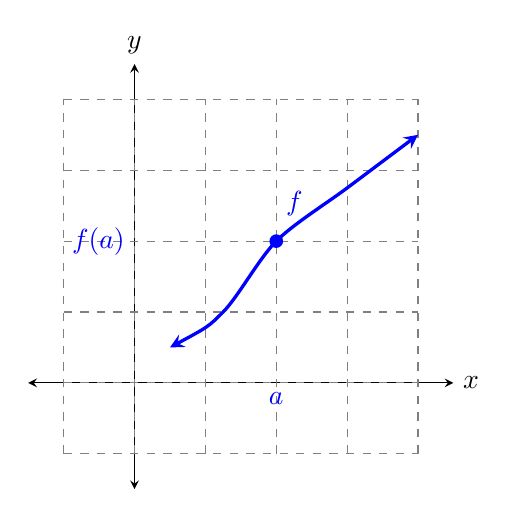
\begin{tikzpicture}[scale=0.9]
    \draw[<->] (-1.5,0) -- (4.5,0) node [right] {$x$};
    \draw[<->] (0,-1.5) -- (0,4.5) node [above] {$y$};
    \draw[color=gray, dashed] (-1,-1) grid (4,4);
    \draw[<->,color=blue,very thick] plot [smooth] coordinates {(0.5,0.5) (1.25,1) (2,2) (3,2.75) (4,3.5)};
    \draw[color=blue,fill=blue] (2,2) circle (2.5pt) node [above right, yshift=0.2cm] {$f$};
    \node at (0,2) [left, color=blue] {$f(a)$};
    \node at (2,0) [below, color=blue] {$a$};
    \end{tikzpicture}
\end{center}
\end{frame}

\begin{frame}{Example 1}
Explain why each graph is \emph{discontinuous} at $x = a$.    \newline\\ (a) \newline\\
\begin{minipage}{0.6\textwidth}
\begin{tikzpicture}[scale=0.85]
    \draw[<->] (-1.5,0) -- (4.5,0) node [right] {$x$};
    \draw[<->] (0,-1.5) -- (0,4.5) node [above] {$y$};
    \draw[color=gray, dashed] (-1,-1) grid (4,4);
    \draw[<->,color=blue,very thick] plot [smooth] coordinates {(0.5,0.5) (1.25,1) (2,2) (3,2.75) (4,3.5)};
    \draw[color=blue,fill=white] (2,2) circle (2.5pt) node [above right, yshift=0.2cm] {$f$};
    % \node at (0,2) [left, color=blue] {$f(a)$};
    \node at (2,0) [below, color=blue] {$a$};
    \end{tikzpicture}
\end{minipage}
\hspace{-0.75cm}
\begin{minipage}{0.3\textwidth}
\onslide<2->{$f(a)$ is not defined.}
\end{minipage}
\end{frame}

\begin{frame}{Example 1}
Explain why each graph is \emph{discontinuous} at $x = a$.    \newline\\ (b) \newline\\
\begin{minipage}{0.6\textwidth}
\begin{tikzpicture}[scale=0.85]
    \draw[<->] (-1.5,0) -- (4.5,0) node [right] {$x$};
    \draw[<->] (0,-1.5) -- (0,4.5) node [above] {$y$};
    \draw[color=gray, dashed] (-1,-1) grid (4,4);
    \draw[<->,color=blue,very thick] plot [smooth] coordinates {(0.5,0.5) (1.25,1) (2,2) (3,2.75) (4,3.5)};
    \draw[color=blue,fill=white] (2,2) circle (2.5pt) node [above right, yshift=0.2cm] {$f$};
    \draw[color=blue,fill=blue] (2,1) circle (2.5pt);
    \node at (2,0) [below, color=blue] {$a$};
    \end{tikzpicture}
\end{minipage}
\hspace{-0.75cm}
\begin{minipage}{0.3\textwidth}
\onslide<2->{$\lim_{x \to a} f(x) \neq f(a)$}
\end{minipage}
\end{frame}


\begin{frame}{Example 1}
Explain why each graph is \emph{discontinuous} at $x = a$.    \newline\\ (c) \newline\\
\begin{minipage}{0.6\textwidth}
\begin{tikzpicture}[scale=0.85]
    \draw[<->] (-1.5,0) -- (4.5,0) node [right] {$x$};
    \draw[<->] (0,-1.5) -- (0,4.5) node [above] {$y$};
    \draw[color=gray, dashed] (-1,-1) grid (4,4);
    \draw[<-,color=blue,very thick] plot [smooth] coordinates {(0.5,0.5) (1.25,1) (2,2)};
    \draw[color=blue,fill=blue] (2,2) circle (2.5pt);
    \draw[->,color=blue,very thick] plot [smooth] coordinates {(2,1) (2.75,1.5) (3.5,2) (4,2.25)};
    \draw[color=blue,fill=white] (2,1) circle (2.5pt);
    \node at (2,0) [below, color=blue] {$a$};
    \end{tikzpicture}
\end{minipage}
\hspace{-1cm}
\begin{minipage}{0.4\textwidth}
\onslide<2->{$\lim_{x\to a^-} f(x) \neq \lim_{x\to a^+} f(x)$}
\end{minipage}
\end{frame}


\begin{frame}{Example 1}
Explain why each graph is \emph{discontinuous} at $x = a$.    \newline\\ (d) \newline\\
\begin{minipage}{0.6\textwidth}
\begin{tikzpicture}[scale=0.85]
    \draw[<->] (-1.5,0) -- (4.5,0) node [right] {$x$};
    \draw[<->] (0,-1.5) -- (0,4.5) node [above] {$y$};
    \draw[color=gray, dashed] (-1,-1) grid (4,4);
    \draw[<-,color=blue,very thick] plot [smooth] coordinates {(0.5,0.5) (1.25,1) (2,2)};
    \draw[color=blue,fill=white] (2,2) circle (2.5pt);
    \draw[->,color=blue,very thick] plot [smooth] coordinates {(2,1) (2.75,1.5) (3.5,2) (4,2.25)};
    \draw[color=blue,fill=white] (2,1) circle (2.5pt);
    \node at (2,0) [below, color=blue] {$a$};
    \end{tikzpicture}
\end{minipage}
\hspace{-1cm}
\begin{minipage}{0.4\textwidth}
\onslide<2->{$\lim_{x\to a^-} f(x) \neq \lim_{x\to a^+} f(x)$}  \\[10pt]
\onslide<3->{$f(a)$ doesn't exist} \\[10pt]
\onslide<4->{$\lim_{x\to a} f(x) \neq f(a)$}
\end{minipage}
\end{frame}

\section{Determine the numbers for which a function is discontinuous}

\begin{frame}{Determine Where Discontinuous}
Functions are discontinuous at points that involve \pause  \newline\\
\begin{itemize}
    \item Holes \newline\\ \pause
    \item Vertical asymptotes \newline\\ \pause
    \item Gaps in $y$-coordinates (left-hand limit $\neq$ right-hand limit)
\end{itemize}
\end{frame}

\begin{frame}{Example 2}
Identify all discontinuities for each.  \newline\\  
(a) \quad $f(x) = \frac{x^2-2x-15}{x-5}$
\begin{align*}
    \onslide<2->{x-5 &= 0} \\[6pt]
    \onslide<3->{x &= 5} \\
\end{align*}

\onslide<4->{The function is discontinuous at $x = 5$.}
\end{frame}

\begin{frame}{Example 2}
    (b) \quad $f(x) = \frac{x^2-6x}{x-6}$
\begin{align*}
    \onslide<2->{x-6 &= 0} \\[6pt]
    \onslide<3->{x &= 6}    \\
\end{align*}
\onslide<4->{The function is discontinuous at $x = 6$}
\end{frame}

\begin{frame}{Example 2}
(c) \quad $g(x) = \begin{cases}
x+1, & \quad x < 2 \\
-x, & \quad x \geq 2
\end{cases}$    \newline\\
\begin{minipage}{0.6\textwidth}
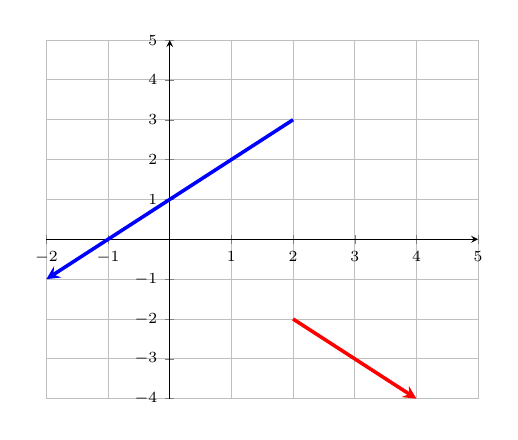
\begin{tikzpicture}[scale=0.8]
\begin{axis}[
axis lines = middle, grid,
xmin = -2, xmax = 5,
ymin = -4, ymax = 5,
xtick = {-2,-1,...,5},
ytick = {-4,-3,...,5}
]
\addplot[<-,color=blue, ultra thick, domain=-2:2] {x+1};
\addplot[->,color=red, ultra thick, domain=2:4] {-x};
\end{axis}
\end{tikzpicture}
\end{minipage}
\hspace{-0.25cm}
\begin{minipage}{0.4\textwidth}
\onslide<2->{Discontinuous at $x = 2$}
\end{minipage}
\end{frame}

\begin{frame}{Example 2}
(d) \quad $g(x) = \begin{cases}
\sqrt{x}, & \quad 0 \leq x < 4 \\
2x, & \quad x \geq 4
\end{cases}$    \newline\\
\begin{minipage}{0.6\textwidth}
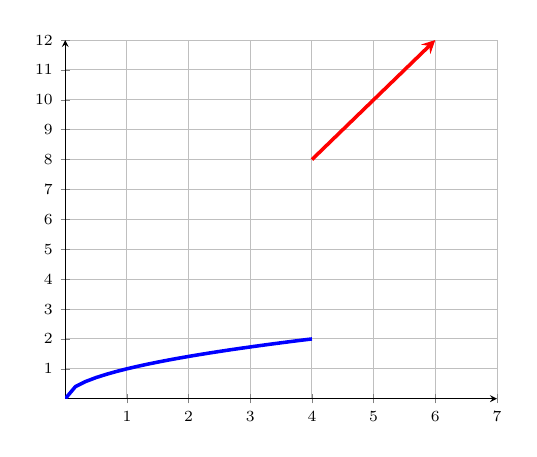
\begin{tikzpicture}[scale=0.8]
\begin{axis}[
axis lines = middle, grid,
xmin = 0, xmax = 7,
ymin = 0, ymax = 12,
xtick = {1,2,...,7},
ytick = {1,2,...,12}
]
\addplot[color=blue, ultra thick, domain=0:4] {sqrt(x)};
\addplot[->,color=red, ultra thick, domain=4:6] {2*x};
\end{axis}
\end{tikzpicture}
\end{minipage}
\hspace{-0.25cm}
\begin{minipage}{0.4\textwidth}
\onslide<2->{Discontinuous at $x = 4$}
\end{minipage}
\end{frame}


\begin{frame}{Example 2}
(e) \quad $f(x) = \begin{cases}
x+1, & \quad x < 2 \\
3, & \quad 2 \leq x < 4 \\
x^2-11, & \quad x \geq 4
\end{cases}$    \newline\\
\begin{minipage}{0.6\textwidth}
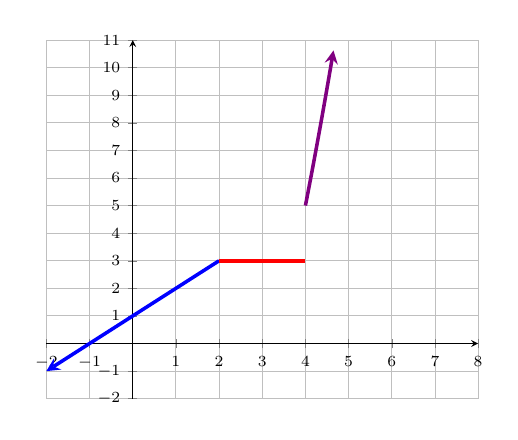
\begin{tikzpicture}[scale=0.8]
\begin{axis}[
axis lines = middle, grid,
xmin = -2, xmax = 8,
ymin = -2, ymax = 11,
xtick = {-2,-1,...,8},
ytick = {-2,-1,...,11}
]
\addplot[<-,color=blue, ultra thick, domain=-2:2] {x+1};
\addplot[color=red, ultra thick, domain=2:4] {3};
\addplot[->,color=violet, ultra thick, domain=4:4.65] {x^2-11};
\end{axis}
\end{tikzpicture}
\end{minipage}
\hspace{-0.25cm}
\begin{minipage}{0.4\textwidth}
\onslide<2->{Discontinuous at $x = 4$}
\end{minipage}
\end{frame}

\begin{frame}{Example 2}
(f) \quad $g(x) = \begin{cases}
\sin x, & \quad x < 0 \\
x^3, & \quad x > 0
\end{cases}$    \newline\\
\begin{minipage}{0.6\textwidth}
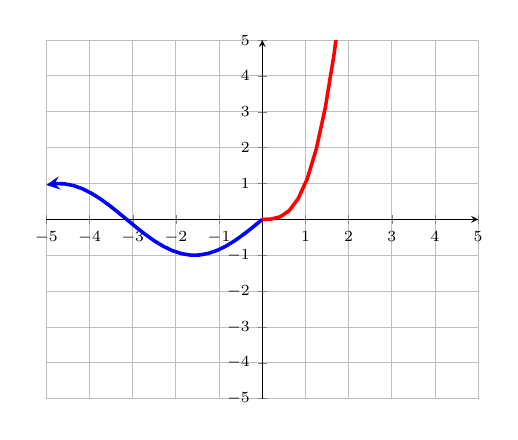
\begin{tikzpicture}[scale=0.8]
\begin{axis}[
axis lines = middle, grid,
xmin = -5, xmax = 5,
ymin = -5, ymax = 5,
xtick = {-5,-4,...,5},
ytick = {-5,-4,...,5}
]
\addplot[<-,color=blue, ultra thick, domain=-5:0] {sin(deg(x))};
\addplot[->,color=red, ultra thick, domain=0:5] {x^3};
\end{axis}
\end{tikzpicture}
\end{minipage}
\hspace{-0.25cm}
\begin{minipage}{0.4\textwidth}
\onslide<2->{Discontinuous at $x = 0$}
\end{minipage}
\end{frame}


\end{document}
